\newcommand{\nom}{Porte conteneur}
\newcommand{\sequence}{03}
\newcommand{\num}{04}
\newcommand{\type}{TD}
\newcommand{\descrip}{Résolution d'un problème en utilisant des méthodes algorithmiques}
\newcommand{\competences}{Alt-C3: Concevoir un algorithme répondant à un problème précisément posé}
\documentclass[10pt,a4paper]{article}
  \usepackage[french]{babel}
  \usepackage[utf8]{inputenc}
  \usepackage[T1]{fontenc}
  \usepackage{xcolor}
  \usepackage[]{graphicx}
  \usepackage{makeidx}
  \usepackage{textcomp}
  \usepackage{amsmath}
  \usepackage{amssymb}
  \usepackage{stmaryrd}
  \usepackage{fancyhdr}
  \usepackage{lettrine}
  \usepackage{calc}
  \usepackage{boxedminipage}
  \usepackage[french,onelanguage, boxruled,linesnumbered]{algorithm2e}
  \usepackage[colorlinks=false,pdftex]{hyperref}
  \usepackage{minted}
  \usepackage{url}
  \usepackage[locale=FR]{siunitx}
  \usepackage{multicol}
  \usepackage{tikz}
  \makeindex

  %\graphicspath{{../Images/}}

%  \renewcommand\listingscaption{Programme}

  %\renewcommand{\thechapter}{\Alph{chapter}}
  \renewcommand{\thesection}{\Roman{section}}
  %\newcommand{\inter}{\vspace{0.5cm}%
  %\noindent }
  %\newcommand{\unite}{\ \textrm}
  \newcommand{\ud}{\mathrm{d}}
  \newcommand{\vect}{\overrightarrow}
  %\newcommand{\ch}{\mathrm{ch}} % cosinus hyperbolique
  %\newcommand{\sh}{\mathrm{sh}} % sinus hyperbolique

  \textwidth 160mm
  \textheight 250mm
  \hoffset=-1.70cm
  \voffset=-1.5cm
  \parindent=0cm

  \pagestyle{fancy}
  \fancyhead[L]{\bfseries {\large PTSI -- Dorian}}
  \fancyhead[C]{\bfseries{{\type} \no \numero}}
  \fancyhead[R]{\bfseries{\large Informatique}}
  \fancyfoot[C]{\thepage}
  \fancyfoot[L]{\footnotesize R. Costadoat, C. Darreye}
  \fancyfoot[R]{\small \today}
  
  \definecolor{bg}{rgb}{0.9,0.9,0.9}
  
  
  % macro Juliette
  
\usepackage{comment}   
\usepackage{amsthm}  
\theoremstyle{definition}
\newtheorem{exercice}{Exercice}
\newtheorem*{rappel}{Rappel}
\newtheorem*{remark}{Remarque}
\newtheorem*{defn}{Définition}
\newtheorem*{ppe}{Propriété}
\newtheorem{solution}{Solution}

\newcounter{num_quest} \setcounter{num_quest}{0}
\newcounter{num_rep} \setcounter{num_rep}{0}
\newcounter{num_cor} \setcounter{num_cor}{0}

\newcommand{\question}[1]{\refstepcounter{num_quest}\par
~\ \\ \parbox[t][][t]{0.15\linewidth}{\textbf{Question \arabic{num_quest}}}\parbox[t][][t]{0.85\linewidth}{#1\label{q\the\value{num_quest}}}\par
~\ \\}

\newcommand{\reponse}[4][1]
{\noindent
\rule{\linewidth}{.5pt}\\
\textbf{Question\ifthenelse{#1>1}{s}{} \multido{}{#1}{%
\refstepcounter{num_rep}\ref{q\the\value{num_rep}} }:} ~\ \\
\ifdef{\public}{#3 ~\ \\ \feuilleDR{#2}}{#4}
}

\newcommand{\cor}
{\refstepcounter{num_cor}
\noindent
\rule{\linewidth}{.5pt}
\textbf{Question \arabic{num_cor}:} \\
}

%%\usepackage[a4paper]{geometry}
%\geometry{margin={1cm,1.2cm}}
%\usepackage[francais]{babel}
%\usepackage{nopageno} %pas de numérotation de page
%\pagestyle{plain} %numérotation en bas de page, pas d'entête
%\usepackage{hyperref}
%\usepackage[latin1]{inputenc}

%%%%%%%%%%%%%%%%%%%%%%%%%%%%%%%%%%%%%%%%%%%%%%%%%%%%%%%%%%%%%%%%%%%%%%%%%%%%%%%%%%%%%

\usepackage{amsthm}
\usepackage{amscd}
%\usepackage{mathrsfs}
%\usepackage{amsfonts}
%\usepackage[T1]{fontenc}
%\usepackage{theorem}
\usepackage{lscape}
\usepackage{variations}  % pour faire des tableaux de variations
\usepackage{dsfont}
\usepackage{fancyvrb} % pour mettre Verbatim dans une box

% Pour les figures
\usepackage{subfig}
%\usepackage{calc} % Pour pouvoir donner des formules dans les d�finitions de longueur
%\usepackage{graphicx} % Pour inclure des graphiques 
% Attention : pour inclure des .jpg comme dans l'exemple (ou des .png ou .pdf)
% il faut compiler directement en pdf (commande pdflatex).
% Pour inclure des .eps, il faut compiler avec latex + dvips + ps2pdf.
\usepackage{psfrag}
%\usepackage{color}

%%%%%%%%%%%%%%%%%%%%%%%%%%%%%%%%%%%%%%%%%%%%%%%%%%%%%%%%%%%%%%%%%%%%%%%%%%%%%%%%%%%%%

\theoremstyle{definition}
\newtheorem*{thm}{Théorème}
%\theorembodyfont{\rmfamily}
\newtheorem*{defn}{Définition}
\newtheorem{exercice}{Exercice}
\newtheorem*{problem}{Problème}
\newtheorem*{prop}{Proposition}
\newtheorem*{corollaire}{Corollaire}
\newtheorem*{lemme}{Lemme}
\newtheorem*{remark}{Remarque}
\newtheorem*{notation}{Notation}
\newtheorem*{ex}{Exemple}
\newtheorem*{ppe}{Propriété}
\newtheorem*{meth}{Méthode}
\newtheorem*{rappel}{Rappel}
\newtheorem*{voca}{Vocabulaire}
\setlength{\columnseprule}{0.5pt}


%%%%%%%%%%%%%%%%%%%%%%%%%%%%%%%%%%%%%%%%%%%%%%%%%%%%%%%%%%%%%%%%%%%%%%%%%%%%%%%%%%%%%

\newcommand{\bi}{\bigskip}
\newcommand{\dsp}{\displaystyle}
\newcommand{\noi}{\noindent}
\newcommand{\ov}{\overline}
\newcommand{\dsum}{\displaystyle \sum}
\newcommand{\dprod}{\displaystyle \prod}
\newcommand{\dint}{\displaystyle \int}
\newcommand{\dlim}{\displaystyle \lim}

%%%%%%%%%%%%%%%%%%%%%%%%%%%%%%%%%%%%%%%%%%%%%%%%%%%%%%%%%%%%%%%%%%%%%%%%%%%%%%%%%%%%%


%\newcommand{\pgcd}{\mathrm{pgcd}} % pgcd
%\providecommand{\norm}[1]{\lVert#1\rVert} % norme
%\DeclareMathOperator{\Tan}{Tan}  % espace tangent


\newcommand{\N}{\mathbb{N}}
\newcommand{\Z}{\mathbb{Z}}
\newcommand{\Q}{\mathbb{Q}}
\newcommand{\R}{\mathbb{R}}
\newcommand{\C}{\mathbb{C}}
\newcommand{\K}{\mathbb{K}}
\newcommand{\U}{\mathbb{U}}
\newcommand{\Tr}{\text{Tr}\,}
\newcommand{\pg}{\geqslant}
\newcommand{\pp}{\leqslant}
\newcommand{\bul}{\item[$\bullet$]}
\newcommand{\card}{\text{Card}}
\newcommand{\re}{\text{Re}\;}
\newcommand{\im}{\text{Im}\;}
\newcommand{\Ker}{\text{Ker}\;}
\newcommand{\Vect}{\text{Vect}\;}
\newcommand{\rg}{\text{rg}\;}
\newcommand{\TT}{{}^t\!}
%\newcommand{\sh}{\text{sh}}
%\newcommand{\ch}{\text{ch}}
\newcommand{\Mat}{\text{Mat}}
\usepackage{textcomp}



%%%%%%%%%%%%%%%%%%%%%%%%%%%%%%%%%%%%%%%%%%%%%%%%%%%%%%%%%%%%%%%%%%%%%%%%%%%%%%%%%%%%%%%%%%%%%%%%%%%%%%%%%%%%%%%%%%%%%%%%%%%




\begin{document}

\begin{center}
{\Large\bf TP \no {\num} -- \descrip}
\end{center}

\section{Démarrage de l'ordinateur et identification}

Lorsqu'on démarre un ordinateur, un ensemble de processus sont mis en œuvre successivement et progressivement jusqu'à ce que la personne désirant utiliser l'ordinateur puisse le faire concrètement. Les principales étapes sont les suivantes :
\begin{enumerate}
 \item Démarrage d'un petit programme, appelé \textit{firmware}\footnote{Il s'agit souvent de BIOS ou de UEFI.} et stocké dans une mémoire dite « morte » (mémoire ROM ou EEPROM) et qui permet notamment d'activer les \textit{périphériques} (écran, clavier, éventuellement souris et périphériques audio). Le \textit{firmware} indique également au \textit{processeur} l'emplacement de la \textit{mémoire de masse} (disque dur ou mémoire flash) dans lequel il doit aller lire les informations relatives au \textit{système d'exploitation} (ou \textit{operating system} « \textit{OS} »).
 
 \textbf{En TP} Vous n'avez pas accès au firmware.
 
 \item Si plusieurs systèmes d'exploitation sont présents, un autre petit programme, le \textit{boot loader} permet parfois à l'utilisateur de choisir lequel il souhaite. Par exemple, certains ordinateurs de la salle informatique peuvent être utilisés sous Ubuntu GNU/Linux et Windows : après le premier écran de démarrage, un menu de systèmes d'exploitation pourrait être proposé à l'utilisateur : il disposerait alors de quelques secondes pour effectuer son choix ; par défaut, si aucune action n'est effectuée, c'est le système Ubuntu GNU/Linux qui est utilisé. 
 
 \textbf{En TP} Cette fonctionnalité a été cachée, vous n'y avez pas accès directement.
 
 
 \item Écran de connexion : le système d'exploitation choisi propose ensuite un écran de connexion, permettant de s'identifier à l'aide d'un nom d'utilisateur et, parfois, d'un mot de passe. Cette étape est cruciale puisqu'à chaque utilisateur ou groupe d'utilisateurs sont associés différents \textit{droits} (lecture, écriture, exécution, possibilité de modifier certaines parties des paramètres du système d'exploitation, etc.). 
 
 \textbf{En TP} Normalement, il n'existe que deux utilisateurs prédéfinis sur les ordinateurs de la salle d'informatique : « professeur » et « élève ». La compte « élève » s'identifie avec le mot de passe « eleve » : sélectionner ce compte, saisir le mot de passe et taper sur « Entrée ».
 
\end{enumerate}

\section{Généralités sur les systèmes d'exploitation / système de fichiers}

Une fois un utilisateur identifié la plupart des OS proposent deux types d'\textit{interfaces système}, c'est-à-dire de façon d'utiliser l'ordinateur :
\begin{enumerate}
 \item une \textit{interface graphique} : c'est celle à laquelle tout le monde est habitué et qui propose des fenêtres, des menus déroulants, des icônes à cliquer, etc. et permettant de lancer des applications (navigateur web, gestionnaire de fichiers, python, etc.) ;
 \item une \textit{interface en mode texte} (ou \textit{interprète de commande}) : elle permet de réaliser les mêmes tâches que l'interface graphique (et même plus !) à partir de commandes tapées au clavier. Bien que non ergonomique et d'apparence un peu désuète et  il s'agit d'une méthode extrêmement robuste et efficace d'utiliser un ordinateur.
\end{enumerate}

\newpage
\section{Interface en mode texte}

\begin{figure}[htp]
 \centering
 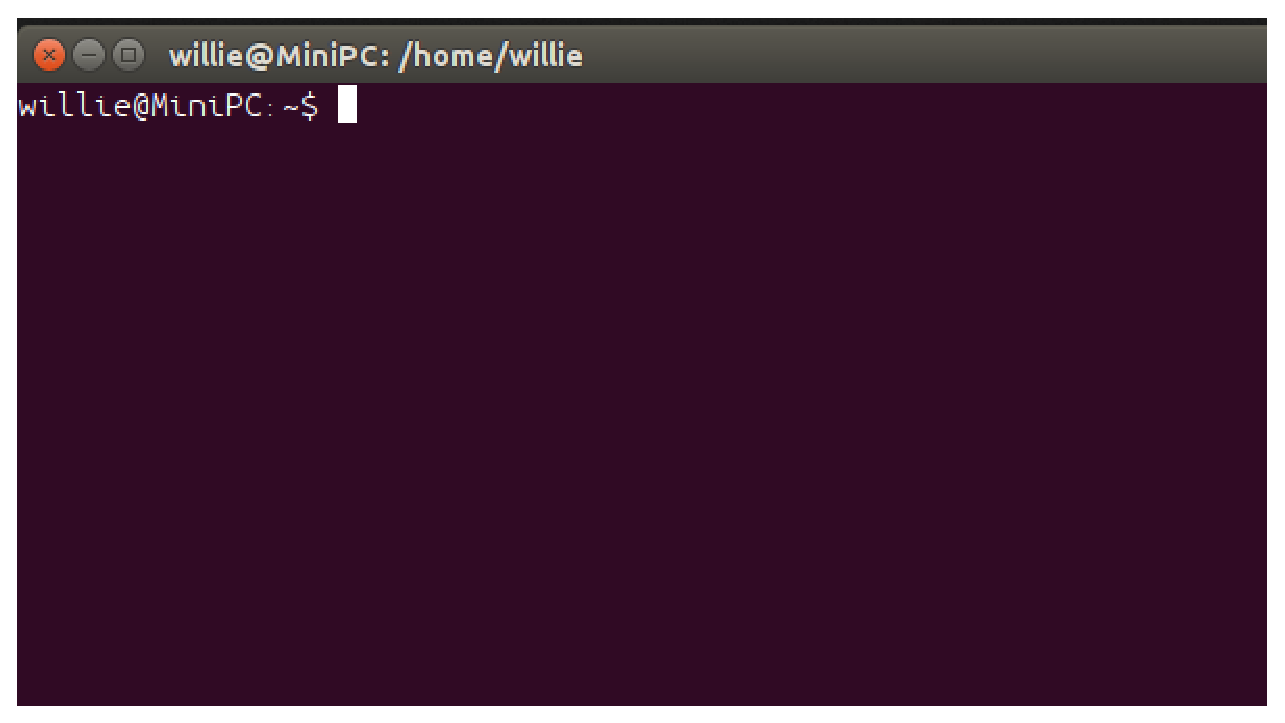
\includegraphics[width=6cm]{img/terminal}
 \caption{Terminal}
 \label{fig:terminal}
\end{figure}

Sous Ubuntu GNU/Linux, vous pouvez accéder à l'émulation d'une interface en mode texte à l'aide d'un terminal (voir figure~\ref{fig:terminal}). 

\textbf{En TP} Taper au clavier la combinaison « Ctrl + Alt + T ». Pour accéder à un terminal. En début de ligne, on voit le nom d'utilisateur connecté et le nom de l'ordinateur. Après le caractère « \$ », il est possible de taper des commandes puis de taper sur « Entrée ». Essayer successivement les commandes suivantes :
\begin{itemize}
 \item[] \texttt{date}
 \item[] \texttt{whoami}
\end{itemize}

\subsection{Commandes de base}
À l'aide de lignes de commande on peut également \textit{naviguer dans le système de fichiers}, c'est-à-dire parcourir l'arborescence des différents dossiers qui structurent les données enregistrées dans la mémoire de masse. Les principales commandes sont :
« \texttt{pwd} » pour savoir dans quel dossier le terminal travaille actuellement ; 
« \texttt{ls} » pour lister les dossiers et fichiers accessibles depuis le dossier actuellement ;
« \texttt{ls -l} » utilise une option permettant de voir de façon ordonnée l'ensemble des informations sur les dossiers et fichiers (les dix premiers caractères regroupent les informations sur le type (dossier, lien, fichier) et sur les droits de lecture, d'écriture, d'exécution ; viennent ensuite : utilisateur propriétaire, groupe propriétaire, horodatage de la dernière modification, nom) ;

Si le premier caractère d'un élément affiché par \texttt{ls -l} est \texttt{d} alors il s'agit d'un sous-dossier du dossier actuel : on peut y faire travailler le terminal en utilisant la commande \texttt{cd} suivie du nom du sous-dossier.

\textbf{En TP} : se familiariser avec la navigation en mode texte dans le système de fichiers en :
\begin{enumerate}
\item repérant le nom d'un sous-dossier et taper la commande adéquate pour y faire travailler le terminal ;
\item tapant « \texttt{cd ..} » pour revenir au dossier immédiatement supérieur ;
\item tapant « \texttt{pwd} » pour connaître le dossier courant.
\end{enumerate}

%gedit, gedit nom de fichier

\subsection{Python dans un terminal}
\label{Python dans un terminal}

Les terminaux permettent également de lancer une session interactive de programmation en python.

\textbf{En TP} : taper \texttt{python} dans votre terminal.

Le terminal affiche un certains nombres d'informations sur python puis un nouveau type de ligne de commande débutée par « > > > ». Vous êtes alors dans une session python, et seules les commandes connues de python sont alors actives et correctement interprétées. À tout moment, pour quitter cette session python, on peut taper \texttt{quit()} puis « Entrée » ou la combinaison \texttt{Ctrl + D}.

La programmation en python sera apprise tout au long de l'année. Dans un premier temps, nous nous servirons de python comme calculatrice.

\newpage
\textbf{En TP} : taper les instructions suivantes toujours suivie de « Entrée » et observer les résultats\dots

\ttfamily
\begin{itemize}
 \item[] a=1
 \item[] type(a)
 \item[] a
 \item[] b=2
 \item[] type(b)
 \item[] b
 \item[] a+b
 \item[] a/b
 \item[] a=1.
 \item[] type(a)
 \item[] a
 \item[] b=2.
 \item[] type(b)
 \item[] b
 \item[] a+b
 \item[] a/b
\end{itemize}

\rmfamily

On comprend assez vite qu'un langage de programmation obéit à des règles strictes qui ne correspondent pas toujours à l'intuition même pour une opération aussi simple qu'une division.

\textbf{En TP} : taper les instructions suivantes toujours suivie de « Entrée » et observer les résultats\dots

\ttfamily

\begin{itemize}
 \item[] 1-3*1/3.
 \item[] 1-1/3.
 \item[] 1-1/3.-1/3.
 \item[] 1-1/3.-1/3.-1/3.
\end{itemize}

\rmfamily

Visiblement l'affichage du résultat des opérations précédentes « cache » quelque chose{\dots} Pour en être sûr, taper :

\begin{minted}[]{python}
from decimal import Decimal
Decimal(1/3.)
\end{minted}

Il va falloir apprendre et comprendre le cours d'Informatique pour interpréter ce comportement un peu particulier de la « calculatrice python\footnote{De la plupart des calculatrices numériques informatisées en réalité. Essayez « 1-1/3-1/3-1/3 » sur votre calculatrice pour en être sûr.} ».

Avant de passer à la partie suivante, quitter python en tapant \texttt{Ctrl + D} puis fermer le fenêtre du terminal.

\section{Environnement intégré de développement : Spyder}

\subsection{L'interface}
Dans un terminal, Python est interpr\' et\' e ligne par ligne. Pour ex\' ecuter plusieurs lignes de commandes, il faut utiliser un \' editeur de fichier. Cette ann\' ee, nous travaillerons avec l'environnement Spyder qui a l'avantage d'\^ etre « userfriendly» .\\
Ouvrez Spyder en le s\' electionnant dans la barre des t\^ aches situ\' ee \` a gauche ou en bas de votre \' ecran.\\
L'interface est d\' ecoup\' ee est trois partie :
\begin{enumerate}
\item en bas \`  a droite : l'interpr\' eteur interactif ou console. Les commandes y sont interpr\' et\' ees ligne par ligne comme dans le terminal, vu \` a la section pr\' ec\' edente.
\item \` a gauche : l'\' editeur de fichier. On y r\' edige les programmes. Les scripts en Python contiennent plusieurs lignes de commandes qui seront ensuite ex\' ecut\' ees.
\item la derni\` ere fen\^ etre ne sera pas utilis\' ee aujourd'hui. Elle permet d'afficher diff\' erents volets qui pourront vous aider dans votre programmation comme : explorateur de variables (indique le type et le nom des variables qui sont utilis\' ees dans votre script), inspecteur d'objets (donne de la documentation sur les fonctions utilis\' ees), ...
\end{enumerate}


\begin{exercice}[Interpr\' eteur interactif]

Reprenez l'exercice de la section \ref{Python dans un terminal} et tapez les lignes de commandes dans l'interpr\' eteur interactif. Vous devez obtenir les m\^ emes r\' esultats.
\end{exercice}


\subsection{R\` egles de sauvegarde d'un fichier}
Avant m\^ eme de commencer \` a r\' ediger un script, il faut le sauvegarder. Quelques r\` egles indispensables :
\begin{enumerate}
\item Toujours v\' erifier \textbf{l'emplacement} de votre sauvegarde. Lors des TP d'informatique, vous devrez sauvegarder vos programmes sur votre clé USB ou \' eventuellement dans un dossier à votre nom dans « /home/eleve/Dossiers personnels » 

Si votre dossier personnel n'existe pas, créez-le : sur le bureau, repérez l'icône « Dossiers personnels », cliquez dessus ; naviguez jusque dans le répertoire « PTSI », faites un clic-droit puis choisissez « Créer un nouveau{\dots} dossier ». Entrez votre NOM suivi de votre Prénom, par exemple : \texttt{MARTIN Jean-Alexandre}. 

\item Nommer de fa\c  con \textbf{pertinente} vos fichiers. Le nom du fichier doit contenir trois informations :
\begin{enumerate}
\item le nom du cr\' eateur du programme (vous) car vous \^ etes nombreux \` a sauvegarder sur la m\^ eme machine,
\item le nom du programme,
\item la version du programme (pour garder une trace des versions successives),
\item l'extension du fichier, séparée du nom du fichier par un « . » : elle indique le type de fichier (par exemple fichier texte, feuille de calcul de tableur, etc.) ; pour un script python, l'extension est « .py ».
\end{enumerate}
\item Pas de ponctuation, d'espace dans le nom d'un fichier. Seul le underscore «\_»   est accept\' e.
\item Le nom d'un fichier sera donc du type :
\begin{center}
NomProgramme\_Version.py\hspace{2cm} Ex : TP1\_JoliDessin\_V1.py
\end{center}
\end{enumerate}


\subsection{Ex\' ecution d'un fichier}

Pour naviguer dans Spyder, vous pourrez utiliser trois m\' ethodes :
\begin{enumerate}
\item en cliquant dans le menu, tout en haut,
\item en cliquant sur la barre d'outils (celle qui contient les petites ic\^ ones),
\item en utilisant les raccourcis clavier.
\end{enumerate}

\begin{exercice}[Cr\' eation d'un fichier] 

\begin{enumerate}
\item Cr\' eer un nouveau fichier en utilisant l'une des trois m\' ethodes (cliquer sur l'ic\^ one correspondante OU aller dans « fichier » OU taper « Ctrl N »)
\item Sauvegarder ce fichier vide en respectant les r\` egles \' enonc\' ees ci-dessus.
\end{enumerate}
\end{exercice}


\begin{exercice}[Ex\' ecution d'un fichier]

\begin{enumerate}
\item Dans votre programme cr\' e\' e pr\' ec\' edemment, recopier le script suivant. On sera attentif \` a la ponctuation et \` a l'indentation.

\begin{minted}[linenos]{python}
from mpl_toolkits.mplot3d import Axes3D
from matplotlib import cm
from array import array   
import matplotlib.pyplot as plt   
import numpy as np   
import csv   
X1 = []   
Y1 = []   
Z1 = []   
cr = csv.reader(open("FICHIER","rb"))   
for row in cr:   
   X1.append(float(row[0]))
   Y1.append(float(row[1]))  
   Z1.append(float(row[2]))
X = np.asarray(X1)   
Y = np.asarray(Y1)   
Z = np.asarray(Z1)   
fig = plt.figure()   
ax = fig.gca(projection='3d')   
surf = ax.scatter(X, Y, Z)   
plt.show()
\end{minted}

\item À la ligne \textbf{10}, le programme va r\' ecup\' erer les donn\' ees pr\' esentes dans le fichier \textit{data.csv}. Il faut indiquer \` a Python l'emplacement de ce fichier. Pour obtenir le chemin d'acc\` es \` a un fichier, il faut parcourir l'arborescence du disque. Sous la plupart des syst\` emes d'exploitation, cela peut \^ etre fait en ouvrant un dossier quelconque puis en naviguant dans les diff\' erents dossiers et sous-dossiers. Sous Ubuntu, l'ic\^ one d\' edi\' ee se trouve dans la barre lat\' erale et prend l'aspect d'un petit dossier appel\' e « Dossier personnel ». Le fichier que nous utiliserons est nomm\' e \textit{data.csv} et est situ\' e dans le dossier \textit{/home/eleve/Ressources/PTSI/TP01/Code}. Se placer dans ce dossier. Faire un clic-droit sur le fichier. Choisir « propri\' et\' es » . S\' electionner et copier le chemin d'acc\` es qui appara\^ it apr\` es «~Emplacement ».
\item Dans votre programme, \` a la place de « FICHIER », coller le chemin d'acc\` es suivi de «/data.csv ».
\item Ex\' ecuter le programme par les trois m\' ethodes :
\begin{enumerate}
\item en cliquant dans le menu sur « Ex\' ecution»  puis « Ex\' ecution » ,
\item en trouvant dans la barre d'outil le bouton « ex\' ecuter le script » ,
\item en trouvant le raccourci clavier.
\end{enumerate}
\end{enumerate}
\end{exercice}

\section{Analyse d'un algorithme}

La suite va consister en l'analyse de l'algorithme d'un test de personnalité. Le fichier est disponible dans le dossier \textit{/home/eleve/Ressources/PTSI/TP01/Code}. Copier-le dans votre répertoire personnel et ouvrez-le avec Spyder. Il doit contenir :

\begin{minted}[linenos]{python}
#!/usr/bin/python 
#Test_personalite.py 
 
questions1 = [("Votre talent tient dans vos", "super-pouvoirs", "ressources"), 
("Un animal est pour vous un", "symbole", "truc pas pratique lorsqu'on part en vacances")] 
result='' 
 
for question in questions1: 
    question_string = "%s:\n\ta. %s\n\tb. %s\n[a/b]:  " % (question[0], question[1], question[2]) 
    answer = raw_input(question_string).lower() 
    while answer not in ("a", "b"): 
        print("Please choose A or B") 
        answer = raw_input(question_string).lower() 
    result = result + answer 
 
if result == 'aa': 
    print 'Vous etes Spiderman !' 
elif  result == 'ab': 
    print 'Vous etes Superman !' 
elif  result == 'ba': 
    print 'Vous etes Batman !' 
else: 
    print 'Vous etes Iron man !'
\end{minted}

\begin{exercice}[Ex\' ecution d'un fichier]

\begin{enumerate}
\item Lancer le programme plusieurs fois en modifiant vos réponses afin de déterminer comment ces réponses influent sur le résultat.

~\

Un organigramme permet de décrire le comportement d'un algorithme. Un exemple simple est présenté ci-dessous.

\begin{minipage}{.2\linewidth}
\ttfamily

\begin{tabbing}
if \= a == b \\
\> do 1 \\
elif a == c \\
\> do 2 \\
else do 3
\end{tabbing}

\rmfamily

\end{minipage}\hfill
\begin{minipage}{.7\linewidth}
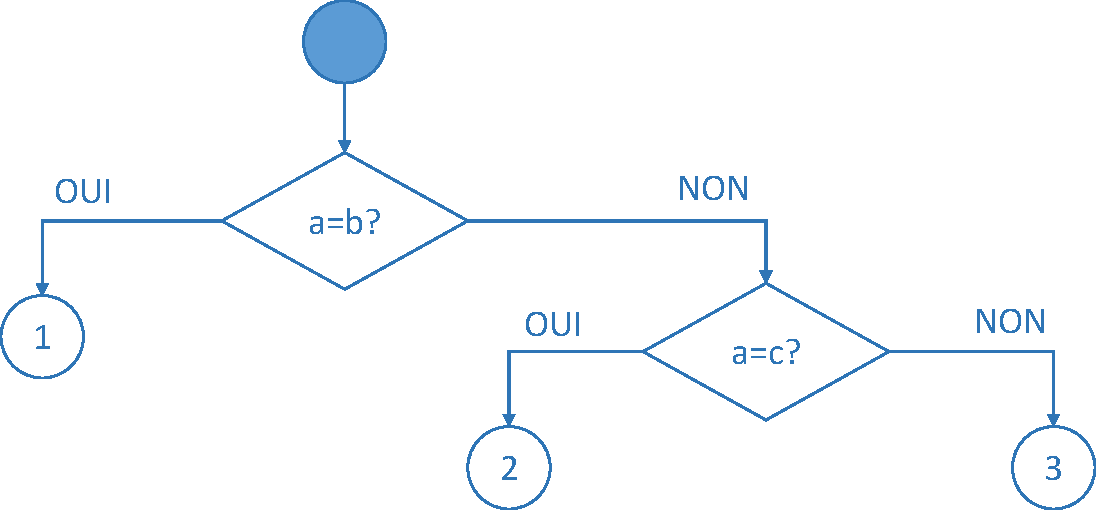
\includegraphics[width=0.6\linewidth]{img/Organigramme}
\end{minipage}
\item Décrire à l'aide de cette représentation le comportement du script précédent.
\item Dans le cas où le résultat est \texttt{'Vous etes Batman !'} quelle est la valeur de la variable \texttt{answer} ?
\item Compléter le questionnaire en ajoutant une question. On commencera par déterminer le nombre de nouveaux super-héros que cela fait apparaitre. \\
Compléter ensuite le questionnaire en ajoutant une proposition \og c \fg pour chaque question afin de faire apparaître de nouveaux super-héros (féminins si possible !).
\end{enumerate}
\end{exercice}

%rajouter question : modifier pour tester le genre et d'autres super heroines

\end{document}
